\documentclass[11pt]{beamer}

\mode<presentation>
{
\usetheme{CambridgeUS}
%\usetheme{IAS_sidebar} 	% only a simple left side bar, frame-title box varies in size when using subtitles for frames.
%\usetheme{IAS_sidebar2_10pt} 	% only a simple side bar, the frame-title box has a fixed size to exactly fit a title and subtitle. For usage with 10pt font, i.e.: \documentclass[10pt]{beamer}
%\usetheme{IAS_sidebar2_11pt} 	% As above only changed to fit 11pt fonts.
%\usetheme{IAS_sidebar2_12pt} 	% As above only changed to fit 12pt fonts.
%\usetheme{IAS_sidebarNav} 	% An IAS side bar with navigation
%\usetheme{IAS_topNav}		% Only top navigation with IAS colors
%\usetheme{IAS_topNav_bottomAuthorTitle}	%Top navigation and author/title in the bottom with IAS colors
%\usetheme{IAS_topNav_leftIASbar_10pt}	% both top navigation and the IAS sidebar, the frame-title box has a fixed size to exactly fit a title and subtitle. For usage with 10pt font, i.e.: \documentclass[10pt,english
%\usetheme{IAS_topNav_leftIASbar_11pt}	% As above only changed to fit 11pt fonts.
%\usetheme{IAS_topNav_leftIASbar_12pt}	% As above only changed to fit 12pt fonts.
  \setbeamercovered{transparent}
%   % or whatever (possibly just delete it)
}

\usepackage{times}
\usepackage[T1]{fontenc}
\usepackage[utf8]{inputenc}
%\usepackage{mathpazo,tgpagella}
\usepackage{amsmath,amssymb,amstext,mathtools,siunitx,marvosym}
\usepackage{media9}
\usepackage{multimedia}


\title[]{First-passage Times for persistent Random Walks}
\author[]{Kevin Klein}
\institute[]
{
Naturwissenschaftlich-Technische Fakultät II \\
- Physik und Mechatronik -  \\
Universität des Saarlandes \\
}
\date[]{Forschungsseminar zur Masterarbeit, 2018}
\subject{Forschungsseminar}

\setbeamertemplate{navigation symbols}{}
%\beamerdefaultoverlayspecification{<+->}


%newcommands%
\newcommand{\todo}[1]{
      {\colorbox{red}{ TODO: #1 }}
}
\newcommand{\todotext}[1]{
      {\color{red} TODO: #1} \normalfont
}


\begin{document}

\begin{frame}
\begin{minipage}[h]{0.49\textwidth}
 
\includegraphics[width=0.5\textwidth]{gfx/SFBlogo.png}
\end{minipage}
\begin{minipage}[h]{0.49\textwidth}
\flushright
 
\includegraphics[width=0.5\textwidth]{gfx/SaarlandUniLogo.png}
\end{minipage}


  \titlepage
\end{frame}


\begin{frame}
  \frametitle{Contents}
  \tableofcontents
  % You might wish to add the option [pausesections]
\end{frame}


\section{Migration and Random Walks}

\begin{frame}
 \frametitle{Active motion}
 Active particles consume energy and turn it into persistent motion.
 \begin{minipage}[h]{0.49\textwidth}
  \centering
  Migrating cell
  \movie[width=0.9\textwidth,height=0.9\textwidth,loop,poster]{}{mov/cell.avi}
  {\newline\tiny P. Maiuri, ..., F. Lautenschläger, ..., Cell 161, p. 374, 2015}
 \end{minipage}
 \begin{minipage}[h]{0.49\textwidth}
  \centering
  Bacillus subtilis
  \movie[width=0.9\textwidth,height=0.9\textwidth,loop,poster]{}{mov/bacillus.avi}
  {\newline\tiny J. Najafi et al., under review (2018)}
 \end{minipage}
\end{frame}


\begin{frame}
 \frametitle{Simplest approach to model migration}
 
 \begin{itemize}
  \item How can we model the movement of microorganisms?
  \item A possible approach: simple 1D random walk (\textit{RW}) on a lattice
 \end{itemize}
 \begin{center}
  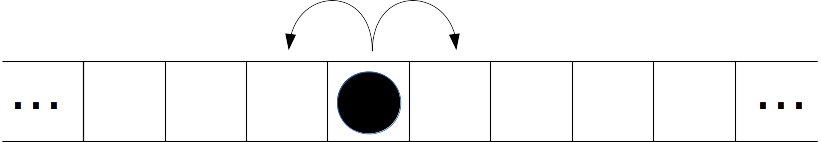
\includegraphics[width=0.9\linewidth]{gfx/1D-SRW.png}
 \end{center} 
 \begin{itemize}
  \item Equal hopping probabilities lead to \textit{diffusion}.
  \item For diffusion the first two moments are:
  \begin{itemize}
   \item $\mathbb{E}\left[X_n\right] = 0$\newline
   \item $\mathbb{E}\left[X^2_n\right] = n$
  \end{itemize}
 \end{itemize}
 
\end{frame}


\begin{frame}
 \frametitle{Random walk with bias}
 
 \begin{itemize}
  \item Asymmetrical hopping rates lead to a bias/drift.
  \end{itemize}
  \begin{center}
   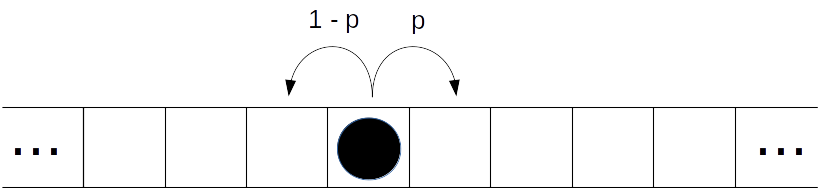
\includegraphics[width=0.9\linewidth]{gfx/1D-BRW.png}
  \end{center}
  \begin{itemize}
    \item Therefore the first two moments are:
    \begin{itemize}
   \item $\mathbb{E}\left[X_n\right] = n\left(2p-1\right)$\newline
   \item $\mathbb{E}\left[X^2_n\right] = n^2$
  \end{itemize}
  \item But here the dispersal about the mean location is more meaningful.
        $\sigma_n \propto n$
  \end{itemize}

\end{frame}


\begin{frame}
 \frametitle{Persistent random walks}
 
 \begin{itemize}
  \item The direction of movement in the previous step influences the hopping probabilites:
 \end{itemize}
 \begin{minipage}[h]{0.49\linewidth}
  \centering
  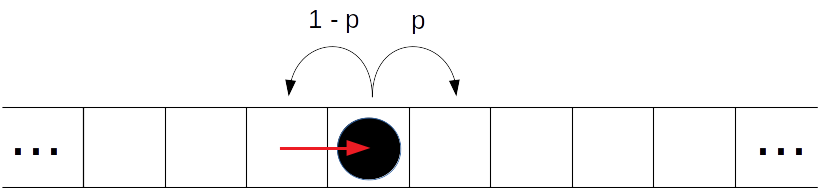
\includegraphics[width=0.9\linewidth]{gfx/1D-PRWright.png}
 \end{minipage}
 \begin{minipage}[h]{0.49\linewidth}
  \centering
  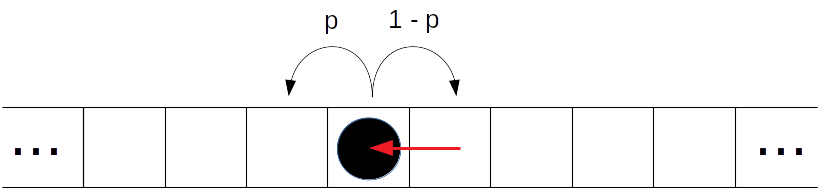
\includegraphics[width=0.9\linewidth]{gfx/1D-PRWleft.png}
 \end{minipage}
 \vspace{1cm}
 \begin{itemize}
  \item In two-dimensional continuous walks: turning angle distribution:
 \end{itemize}
 \begin{center}
  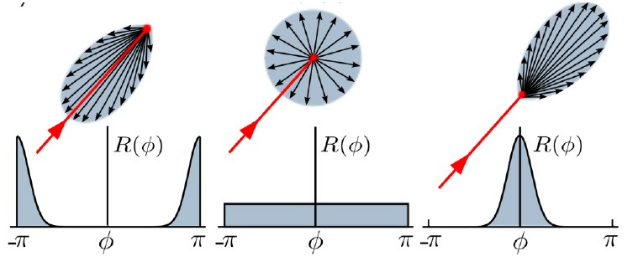
\includegraphics[width=0.6\linewidth]{gfx/turningAngleDistribution.png}
  %\captionof{figure}{\textit{M. R. Shaebani et al., Physical Review E90, 030701, 2014}}
  {\newline\tiny M. Reza Shaebani et al., Phys. Rev. E 90, 030701, 2014}
 \end{center}

\end{frame}


\begin{frame}
 \frametitle{Some properties}
 

  \begin{itemize}
  \item $\mathbb{E}\left[X_n\right] = 0$
  \item For the MSD one obtains:
  $\mathbb{E}\left[X_n^2\right] = \frac{1+p}{1-p}n+\frac{2p}{\left(1-p\right)^2}\left(p^n-1\right)$
  \item Therefore longterm: diffusion
  \item Shortterm: $\mathbb{E}\left[X_n^2\right] \propto n^\alpha$ with
  $\alpha = 1 + \ln\left(1+p\right) / \ln 2$
  \end{itemize}
  \centering
  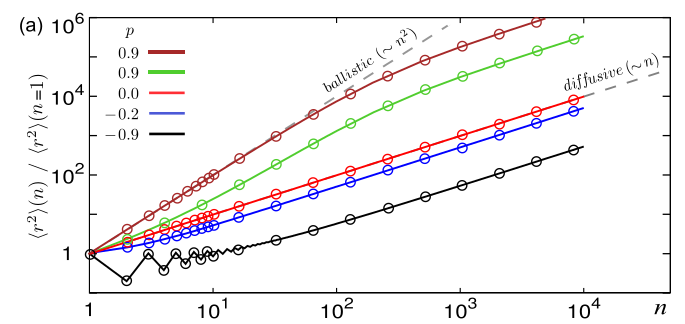
\includegraphics[width=0.7\linewidth]{gfx/msd.png}
 {\newline\tiny M. Reza Shaebani et al., Phys. Rev. E 90, 030701, 2014}
\end{frame}



\begin{frame}
 \frametitle{A 2D lattice model}
 
 \begin{minipage}[h]{0.39\textwidth}
  \centering
  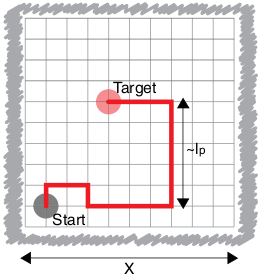
\includegraphics[width=0.9\textwidth]{gfx/search-trajectory.png}
  {\tiny Tejedor et al., Phys. Rev. Lett. 108, 088103, 2012}
 \end{minipage}
 \begin{minipage}[h]{0.59\textwidth}
  \begin{itemize}
   \item 2 dimensional lattice
   \item Periodic boundary conditions
   \item System size of $X \gg 1$
   \item Persistent direction with $p_1$
   \item Other directions with $p_2 =\frac{1 - p_1}{3}$
  \end{itemize}
 \end{minipage}
 \begin{itemize}
  \item Therefore $P\left(l\right) = \left(1-p_1\right) p_1^{l-1}$
  \item Persistence length $l_p = \sum^\infty_{l=1} lP\left(l\right)=\frac{1}{1-p_1}$
 \end{itemize}

\end{frame}


%%%%%%%%%%%%%%%%%%%%%%%%%%%%%%%%%%%%%%%%%%%%%%%%%%
%%%%%%%%%%%%%%%%%%%%%%%%%%%%%%%%%%%%%%%%%%%%%%%%%%
%%%%%%%%%%%%%%%%%%%%%%%%%%%%%%%%%%%%%%%%%%%%%%%%%%
%%%%%%%%%%%%%%%%%%%%%%%%%%%%%%%%%%%%%%%%%%%%%%%%%%
%%%%%%%%%%%%%%%%%%%%%%%%%%%%%%%%%%%%%%%%%%%%%%%%%%
\section{Mean First-Passage Times}

\begin{frame}
 \frametitle{Motivation}
 
 \begin{minipage}[h]{0.5\linewidth}
  \begin{itemize}
   \item Microorganisms need to migrate in order to adapt to environmental changes:
   \begin{itemize}
    \item Finding nutrients
    \item Finding target organisms
    \item Escaping hazardous locations
    \item Relocation for various other biological tasks
   \end{itemize}
   \item An important measure is the time needed to find places of interest.

  \end{itemize}
 \end{minipage}
 \begin{minipage}[h]{0.45\linewidth}
   \centering
   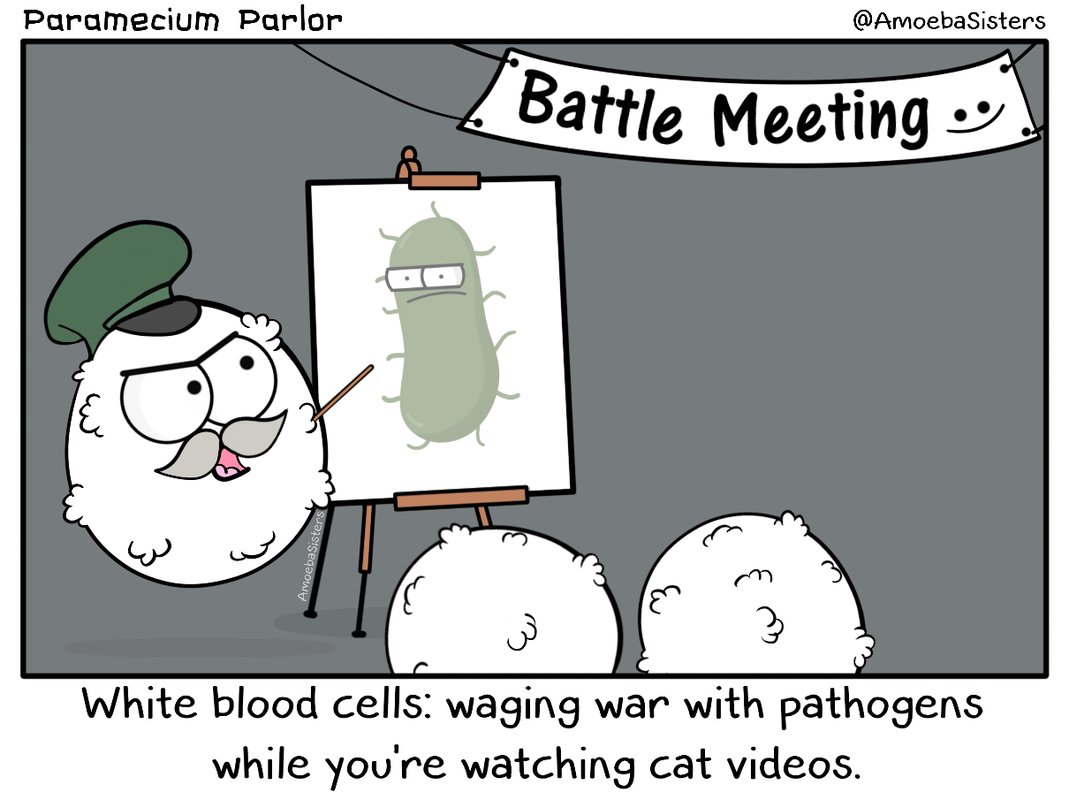
\includegraphics[width=1.0\linewidth]{gfx/white-blood-cell-battle-meeting_orig.png}
 \end{minipage}

\end{frame}


\begin{frame}
 \frametitle{First-passage time}
 
 \begin{minipage}[h]{0.49\textwidth}
  \begin{itemize}
  \item How to define the efficiency of a search?
  \item Time or number of steps it takes to find a hidden target
  \item Mathematically described by the mean first-passage time (MFPT).
 \end{itemize}
 \end{minipage}
 \begin{minipage}[h]{0.49\textwidth}
  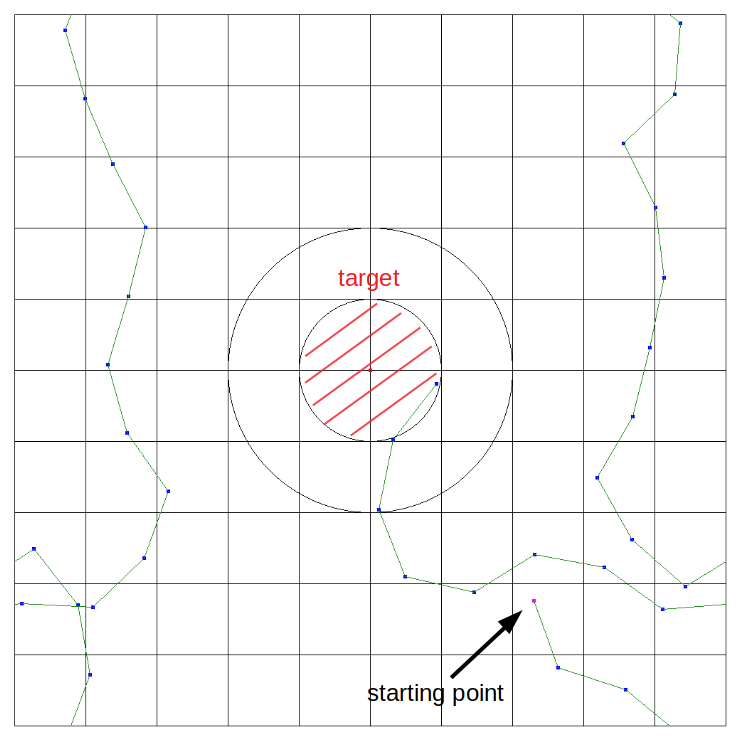
\includegraphics[width=\textwidth]{gfx/trajectory.png}
 \end{minipage}

\end{frame}


\begin{frame}
 \frametitle{Sources of complexity}
 \begin{itemize}
  \item Different types of searches:
  \begin{itemize}
   \item Diffusion
   \item Lévy-Walk
   \item Intermittent (``Run and Tumble'')
   \item Single-state search strategy
  \end{itemize}
  \item Parameters:
   \begin{itemize}
  \item Persistency
  \item System size
  \item Step length / velocity
  \item Size of target / detection range
  \item Information in the environment
  \item Crowded environment
  \item Interactions between targets and/or searchers
 \end{itemize}
 \end{itemize}
\vspace{0.5cm}
\huge$\rightarrow$ \normalsize Simple model with constant persistency
\end{frame}



\section{Results of a Minimal 2D Model}
\begin{frame}
 \frametitle{MFPT of a persistent walker on a 2D lattice}
 \begin{itemize}
  \item Reminder: $l_p = \frac{1}{1-p}$
  \item By using backward equations and fourier transform an exact expression for the MFPT $\tau$ is obtained.
 \end{itemize}
 \begin{minipage}[h]{0.6\textwidth}
  \centering
   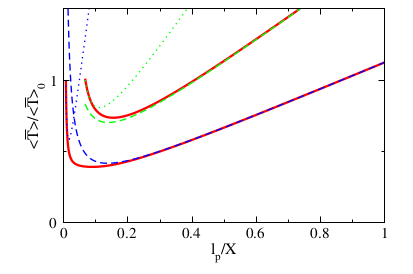
\includegraphics[width=0.9\linewidth]{gfx/mfpt-exact.png}
 \end{minipage}
 \begin{minipage}[h]{0.39\textwidth}
 \begin{itemize}
  \item Upper set of curves: $X=10$
  \item Lower set of curves: $X=100$
  \item Red line: exact results
  \item Dotted/dashed lines: limits
 \end{itemize}
 \end{minipage}
 \begin{itemize}
  \item Search time can be minimized by selecting optimal persistency $p$.
 \end{itemize}
 \centering
 {\tiny Tejedor et al., Phys. Rev. Lett. 108, 088103, 2012}
\end{frame}


\begin{frame}
 \frametitle{Comparison to Lévy walk}
 
 \begin{minipage}[h]{0.49\textwidth}
  \begin{itemize}
  \item Tejedor et al. compare their results to Lévy walk strategies.
  \item One target and system size $X=50$
  \item For the Lévy walk: $P\left(l\right) \propto \frac{1}{l^{1+\mu}}$, with $\mu \in \{1.2, 1.4, 1.6, 1.8, 2\}$ from top to bottom
 \end{itemize}
 \end{minipage}
 \begin{minipage}[h]{0.49\textwidth}
  \centering
  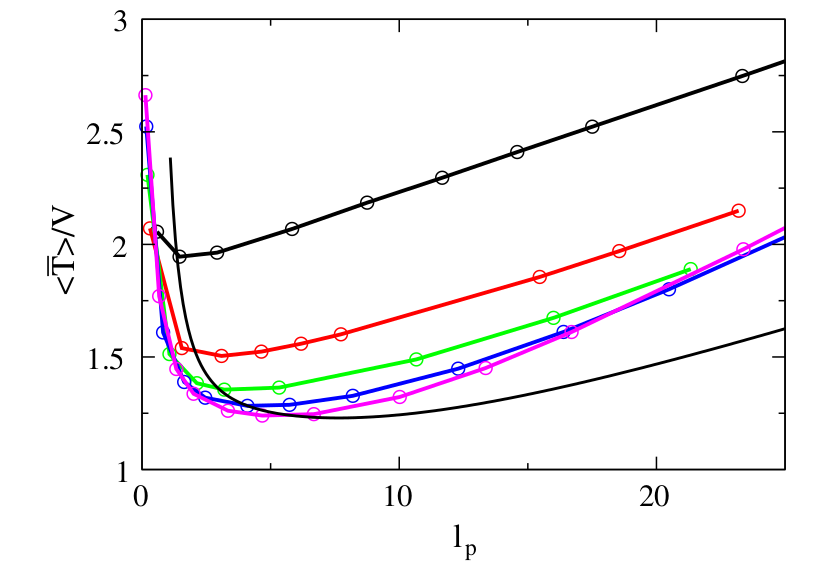
\includegraphics[width=\textwidth]{gfx/tejedor-levywalk.png}
 \end{minipage}
 \begin{itemize}
  \item The persistent random walk with constant state outperforms the Lévy walk strategy here if only one target is available.
 \end{itemize}
\centering
 {\tiny Tejedor et al., Phys. Rev. Lett. 108, 088103, 2012}
\end{frame}


\begin{frame}
 \frametitle{Summary I}
 
 \begin{itemize}
  \item Microorganisms do need to efficiently migrate.
  \item This migration can be modeled by different types of random walks.
  \item The mean first-passage time is an important measure for the efficiency of a search.
  \item Even using a simple search strategy the MFPT can be minimized.
 \end{itemize}

\end{frame}


\section{Non-trivial Search Strategies}

\begin{frame}
 \frametitle{Variable activity}
 
 \begin{itemize}
  \item In biological systems microorganisms show activity.
  \item This activity can be expressed by the persistency $p$.
  \item But why do organisms show activity?
 \end{itemize}

\end{frame}


\begin{frame}
 \frametitle{Hidden vs. visible targets}
 
 \begin{minipage}[h]{0.59\textwidth}
  \begin{itemize}
  \item There might be information about the target location available in the environment.
  \item This information can be sensed by the searcher and therefore it can adapt its activity accordingly.
  \item One can distinguish between deterministic and stochastic navigation.
 \end{itemize}
 \end{minipage}
 \begin{minipage}[h]{0.4\textwidth}
  \centering
  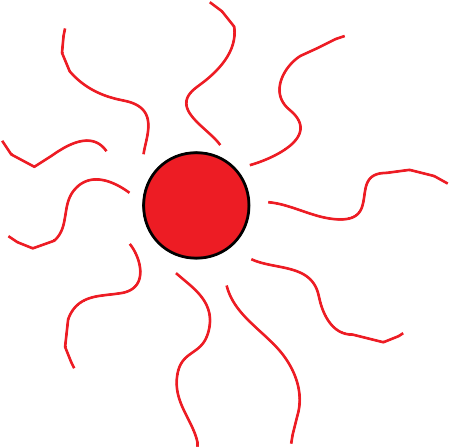
\includegraphics[width=0.8\textwidth]{gfx/smell.png}
 \end{minipage}

\end{frame}


\begin{frame}
 \frametitle{Deterministic navigation}
 
 \begin{itemize}
  \item Local gradient is used to determine the right direction to the target.
  \item E.g.: Chemotaxis, gravitaxis, thermotaxis, magnetotaxis, ...
  \item The tactical response to any information profile is of interest.
 \end{itemize}

\end{frame}


\begin{frame}
 \frametitle{E. coli - Precision vs. motility}
 
 \begin{itemize}
  \item Chemotaxis signal transmission pathway is modified.
  \item Population A has exponentially distributed lengths of runs.
  \item Population B has power-law distributed lengths of runs.
 \end{itemize}

 
 \begin{minipage}[h]{0.49\textwidth}
  \centering
  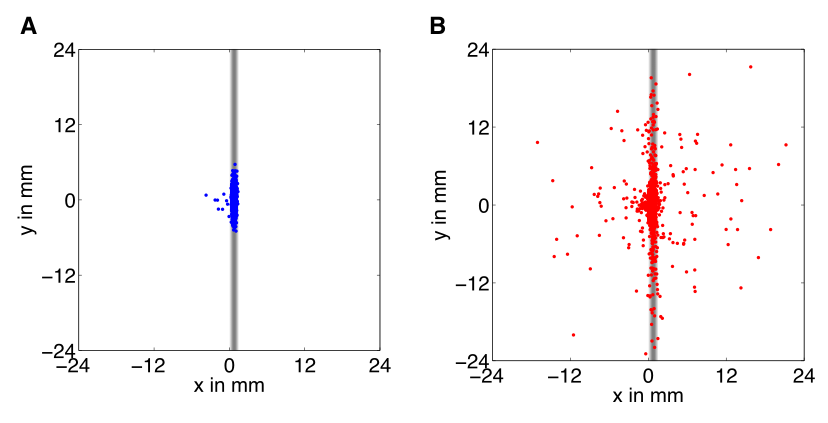
\includegraphics[width=\textwidth]{gfx/trapez.png}
 \end{minipage}
  \begin{minipage}[h]{0.49\textwidth}
  \centering
  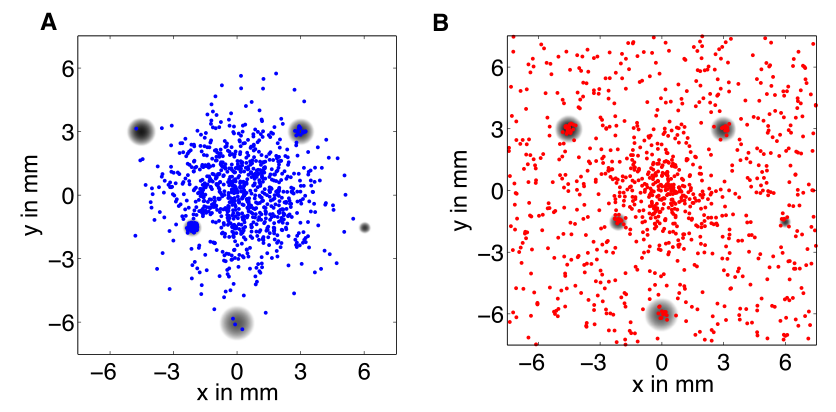
\includegraphics[width=\textwidth]{gfx/dots.png}
 \end{minipage}
 \begin{itemize}
  \item Different behavior/responses advantageous in different scenarios.
 \end{itemize}

 \begin{center}
  {\tiny F. Matthäus et al., Biophysical Journal 97, p. 946, 2009}
 \end{center}
\end{frame}


\begin{frame}
 \frametitle{E. coli chemoattractant profiles and Robot-Infotaxis}
 
 \begin{minipage}[h]{0.64\textwidth}
  \begin{itemize}
   \item Rapidly fluctuating, diverse/complex environments: chemotaxis or shutting down signaling pathway preferable?
   \item Chemotactic response: bias in fraction of time spent in run/tumble.
  \end{itemize}
  \centering
  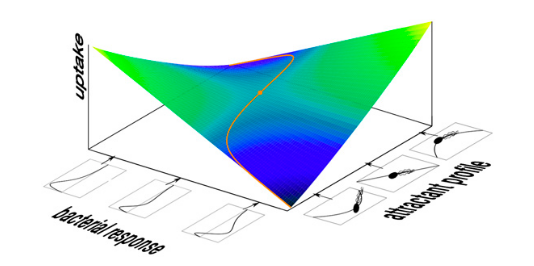
\includegraphics[width=0.9\textwidth]{gfx/responseprofile.png}
  \begin{itemize}
   \item ``Maximin'' strategy always outperforms motile but nonchemotactic bacteria.
  \end{itemize}
  {\tiny A. Celani, M. Vergassola, PNAS 107, p. 1391, 2010}
 \end{minipage}
 \begin{minipage}[h]{0.35\textwidth}
  \centering
  Infotaxis
  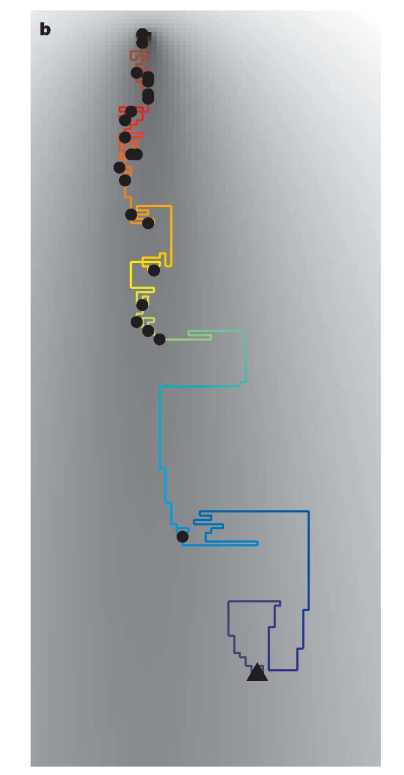
\includegraphics[width=0.8\textwidth]{gfx/infotaxis.png}
  {\newline\tiny M. Vergassola et al., nature 445, p. 406, 2007}
 \end{minipage}
\end{frame}

\begin{frame}
 \frametitle{Stochastic navigation}
 \begin{minipage}[h]{0.59\textwidth}
  \begin{itemize}
   \item Shouldn't deterministic navigation lead straight to the target?
   \item There are several confounding factors:
   \begin{itemize}
    \item Weak gradients or chaotic fields
    \item Sparse information / no gradient
    \item External (and internal) noise
    \item Wrong navigation caused by ligand-receptor binding
   \end{itemize}

  \end{itemize}
 \end{minipage}
\begin{minipage}[h]{0.4\textwidth}
 \centering
 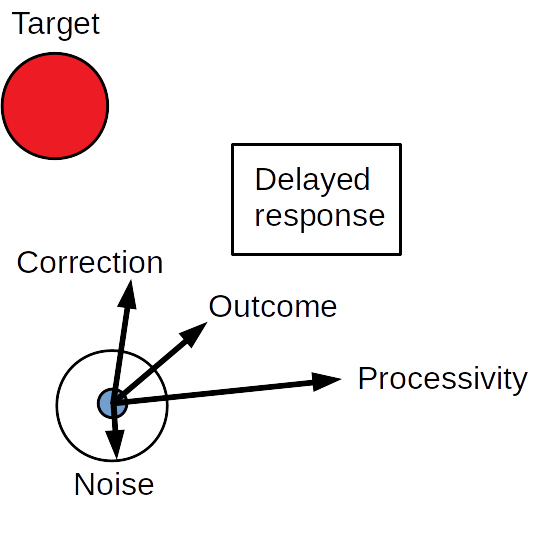
\includegraphics[width=\textwidth]{gfx/chemotrouble.png}
\end{minipage}
\begin{itemize}
 \item Under such conditions it is reasonable to give up on deterministically chosing a direction.
 \item Therefore, directions will be chosen randomly and only the activity changes.
\end{itemize}


 
\end{frame}

\section{Preliminary Results}


\begin{frame}
 \frametitle{Implementation of chemokinesis}
 
 \begin{minipage}[h]{0.49\textwidth}
   \begin{itemize}
   \item For now: 2D lattice model
  \item We assume simple dependencies between distance and persistency.
  \item After each step the persistency is adapted according to the new distance to the target.
  \item Therefore, the movement patterns vary from diffusive to ballistic motion.
 \end{itemize}
 \end{minipage}
 \begin{minipage}[h]{0.49\textwidth}
  \centering
  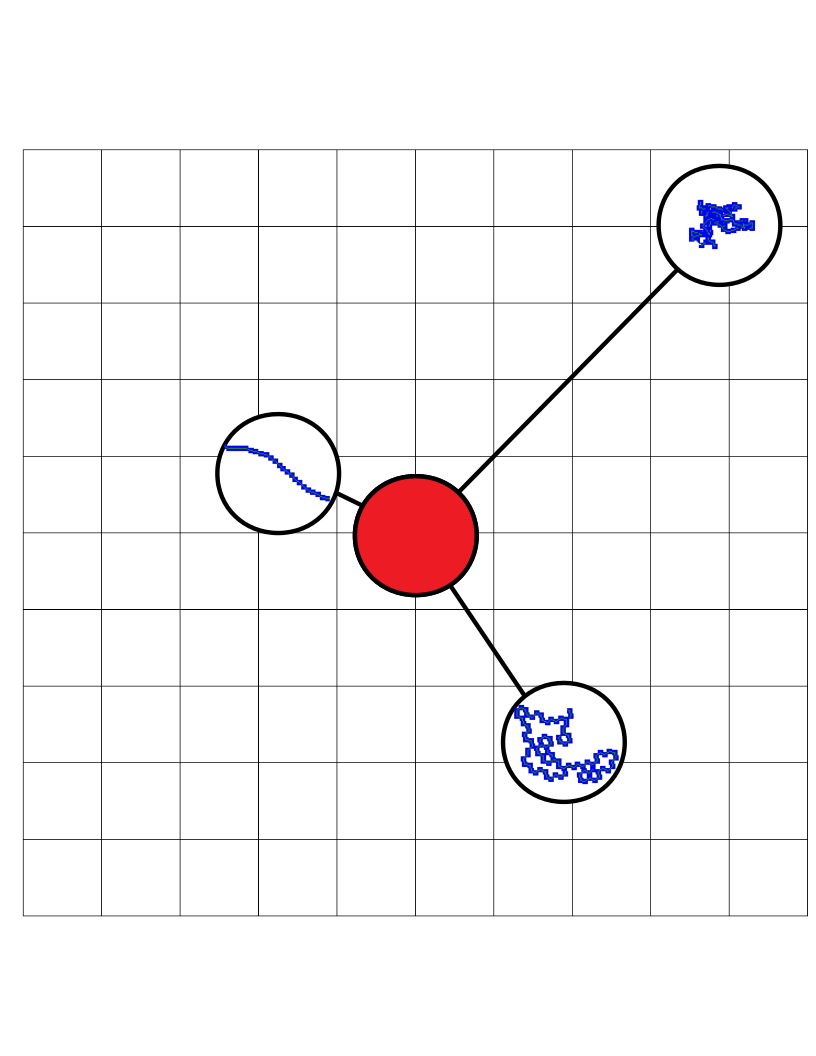
\includegraphics[width=0.9\textwidth]{gfx/profileScheme.png}
 \end{minipage}
\end{frame}


\begin{frame}
 \frametitle{Results - Linear profile}
 
 \begin{itemize}
  \item Linear distance-persistency relation:\newline
        $p\left(d\right)=p_{max}-\left(p_{max}-p_{min}\right)\cdot\frac{\sqrt{2}}{X}\cdot d$
 \end{itemize}
 \begin{minipage}[h]{0.49\textwidth}
  \centering
  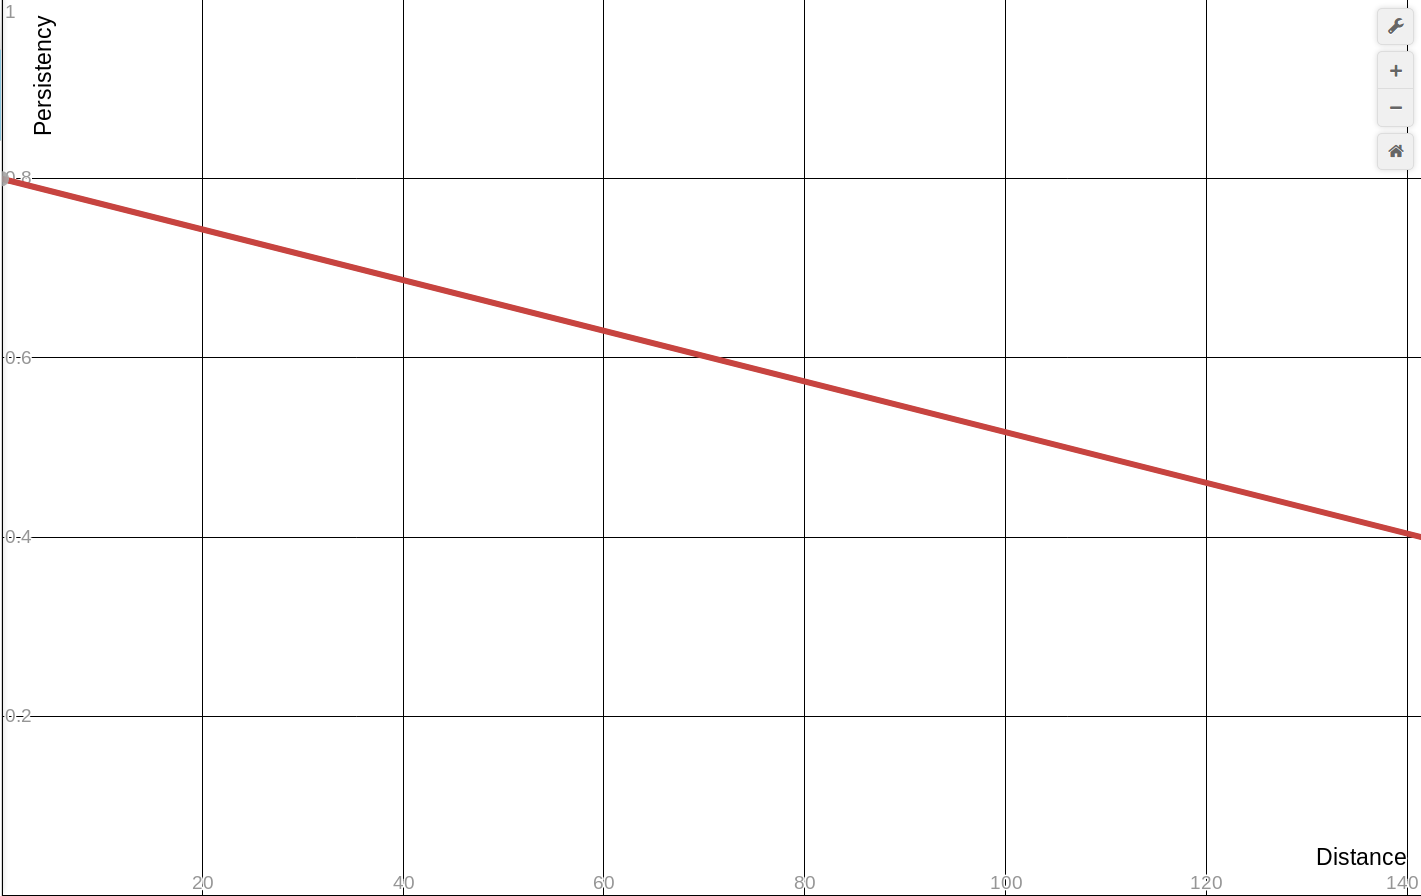
\includegraphics[width=1.0\textwidth]{gfx/linearProfile.png}
 \end{minipage}
 \begin{minipage}[h]{0.49\textwidth}
  \centering
  \includegraphics[width=1.0\textwidth]{gfx/linMFPT-3D.png}
 \end{minipage}
 \begin{itemize}
  \item Parameter sets close to (1,1) outperform constant search strategy
 \end{itemize}
\end{frame}


\begin{frame}
 \frametitle{Results - Parabolic profile}
 
 \begin{itemize}
  \item Parabolic distance-persistency relation:\newline
        $p\left(d\right)=p_{max}-\left(p_{max}-p_{min}\right)\cdot\left(\frac{2\sqrt{2}}{X}\right)^2\cdot \left(d-\frac{X}{2\sqrt{2}}\right)^2$
 \end{itemize}
 \begin{minipage}[h]{0.49\textwidth}
  \centering
  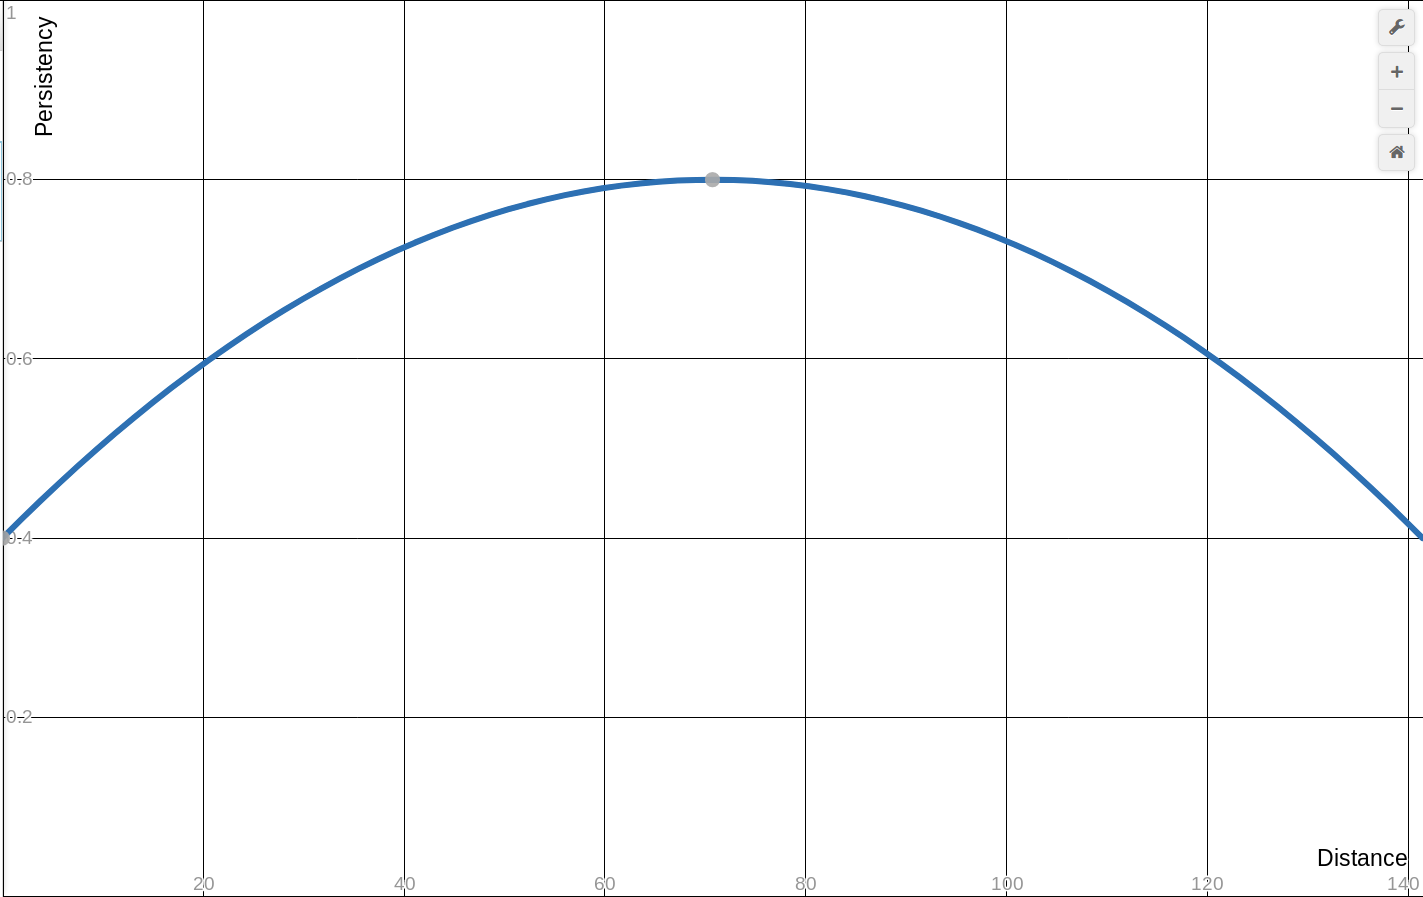
\includegraphics[width=1.0\textwidth]{gfx/parabolProfile.png}
 \end{minipage}
 \begin{minipage}[h]{0.49\textwidth}
  \centering
  \includegraphics[width=1.0\textwidth]{gfx/paraMFPT-3D.png}
 \end{minipage}
 \begin{itemize}
  \item Parameter sets close to (1,1) outperform constant search strategy
 \end{itemize}
\end{frame}


\section{Outlook and Summary}
\begin{frame}
 \frametitle{Outlook}
 
 \begin{itemize}
  \item The preliminary results (as well as other not shown results) suggest to consider the regime of high persistence search in more detail.
  \item Considering the persistence length / higher resolution of p.
  \item Also other mathematical relations between persistency and target-distance need to be explored.
  \item Identify properties of efficient profiles.
  \item Consider a continuous chemokinesis model.
 \end{itemize}

\end{frame}

\begin{frame}
 \frametitle{Summary}
 
 \begin{itemize}
  \item Microorganisms need to efficiently search for targets or locations of interest.
  \item There are different search strategies with their own specific advantages, e.g.:
  \begin{itemize}
   \item Run and tumble
   \item Single-state (constant persistency)
   \item Chemotaxis (gradient)
   \item Chemokinesis (concentration)
  \end{itemize}
  \item Search strategies with concentration/distance dependent persistency can be a useful strategy in order to minimize search times.
 \end{itemize}

\end{frame}





\end{document}
